
%%%%%%%%%%%%%%%%%%%%%%%%%%%%%%%%%%%%%%%%%%%%%%%%%%%%%%%%%%%%%%%%%%%%%%%%%%%%%%%
%
% Nicole's Thesis, IIT 2018
%
%%%%%%%%%%%%%%%%%%%%%%%%%%%%%%%%%%%%%%%%%%%%%%%%%%%%%%%%%%%%%%%%%%%%%%%%%%%%%%%
\documentclass{iitthesis}

% Document Options:
%
% Note if you want to save paper when printing drafts,
% replace the above line by
%
%   \documentclass[draft]{iitthesis}
%
% See Help file for more about options.

\usepackage[dvips]{graphicx}    % This package is used for Figures
\usepackage{rotating}           % This package is used for landscape mode.
\usepackage{epsfig}
\usepackage{subfigure}          % These two packages, epsfig and subfigure, are used for creating subplots.
\usepackage{siunitx}

%% Only for editing process...TAKE OUT for FINAL DRAFT
\usepackage{graphicx,xcolor,enumitem}
\newcommand{\lsnote}[1]{\textsf{{\color{violet}{ LS note:}   #1 }}}
\newcommand{\nrnote}[1]{\textsf{{\color{blue}{ NN note:}   #1 }}}
\newcommand{\jpnote}[1]{\textsf{{\color{green}{ JP note:}   #1 }}}

\begin{document}

\title{Design for Staged Two Beam Acceleration at the Argonne Wakefield Accelerator Facility}

\author{Nicole Neveu }
\degree{Doctor of Philosophy}
\dept{Physics}
\date{May 2018}
\copyrightnoticetrue      % crate copyright page or not
%\coadvisortrue           % add co-advisor. activate it by removing % symbol to add co-advisor
\maketitle                % create title and copyright pages


\prelimpages         % Settings of preliminary pages are done with \prelimpages command

%%%  Acknowledgement %%%
\begin{acknowledgement}     % acknowledgement environment, this is optional
	\par  Family, Lalo, Linda, John, AWA group, Jeff
	%\input{ackno.tex} % you need a separate acknowledgement.tex file to include it.
\end{acknowledgement}

% Table of Contents
\tableofcontents
\clearpage

% List of Tables
\listoftables

\clearpage

%List of Figures
\listoffigures

\clearpage

%List of Symbols(optional)

\listofsymbols
\SymbolDefinition{$c$}{Speed of Light}
\SymbolDefinition{$\epsilon$}{Dielectric Permittivity}
\SymbolDefinition{$\epsilon$}{6D Phase Space Emittance}
\SymbolDefinition{$\gamma$}{Relativistic Kinetic Energy}

\clearpage

%%% Abstract %%%
\begin{abstract}           % abstract environment, this is optional
	\par Staged two beam acceleration using dielectric structures has yet to 
	be achieved anywhere in the world. In this thesis, I discuss the beam 
	line design and simulation, followed by experimental results of a 
	beam line with the potential for dielectric TBA.   
\end{abstract}

\textpages     % Settings of text-pages are done with \textpages command

\Chapter{INTRODUCTION}

\Section{Motivation} \label{sec:motivation}

If there is ever a new generation of accelerators dedicated to High Energy Physics
(HEP), they will be of the TeV scale. Reduction in the size and cost
of such machines is key to their feasibility, and can be accomplished
through accelerator technology R\&D. Investigation into a 
high gradient candidate for future HEP machines was underway
at the Argonne Wakefield Accelerator (AWA) facility. A
short pulse, two-beam acceleration (TBA) scheme using 
wakefield power extractors, and accelerating structures made 
of metallic materials was designed. 
The goal of AWA is to demonstrate a gradient of
\SI{250}{MV/m}, using a TBA dielectric scheme. If successful, this would
be the only facility in the world capable of such gradients used for
acceleration of a beam.

Despite the advantage of higher gradients, there is still experimental work
needed to prove dielectric TBA is a viable candidate for implementation at an HEP or user facility.
TBA requires a drive beam to pass through a decelerating structure and
lose energy through wakefield generation. The electromagnetic wake
is coupled from the decelerator into an accelerating structure, where
the electric field is used to accelerate a second beam. This requires
two complete and separate beamlines operating synchronously with each other.  
The wakefield structures can be metallic or dielectric. Dielectric
structures, having no irises, are simple to manufacture and have demonstrated
high gradient capability at \SI{100}{MV/m} \cite{WeiPaper}. 

The Compact Linear Collider (CLIC) collaboration, proposes a similar TBA scheme with
a \SI{240}{ns} pulse design. This limits the acceleration gradient
to roughly \SI{150}{MV/m} at room temperature due to rf breakdown \cite{CLICdesignReport}.
Higher gradients could be reached when driven by a very short drive
beam pulse, such as the 20ns pulse length proposed by AWA \cite{WeiPaper}. 
\nrnote{Understand and explain why short pulse can give higher gradients. 
Because higher peak power is tolerable, but average power stays the same?}
While the two groups vary on approach, it is agreed that TBA would 
require less infrastructure when constructing a linear TeV scale machine, 
versus the cost of more conventional technology. 
For example, a case study was done using traditional \SI{50}{MW} klystron sources.
It would take roughly 35,000 klystrons to construct a linear machine to deliver the same 
\SI{9.2}{TW} power specification in CLIC reports \cite{CLICdesignReport}. 
In comparison to CLIC's 48 km projected length to reach \SI{3}{TeV}, the Next Linear
Collider (NLC) collaboration projected a length of \SI{26}{km} using X-band klystrons,
only to reach an energy of \SI{1}{TeV}. %\cite{NLC}. 
The power supplied to the witness beam in TBA is similar to
power provided by traditional accelerator technology. 
The key difference is the amount of infrastructure and cost 
needed to transport the power. Theoretically, TBA can deliver
the same amount of power as conventional methods with less 
infrastructure, and therefore lower cost, in the case of a high energy machine. 

Before a true study of the power and infrastructure trade offs 
can be done, the feasibility of staged TBA must be understood, 
as no high energy machine can be built with out a staging.
Staging is the ability to use two accelerating modules back to back to accelerate 
the same particle bunch. While simple in principle, the difficulties 
to achieve staging should not be underwritten. Demonstration of staging proves 
that a TBA scheme can be scaled to high energies, and whether it is 
feasible to use such methods. Single stage TBA, and staging 
in a simplified scheme have been demonstrated at the AWA in 2016.
\nrnote{Not any more? - Demonstration of the full-scale dielectric staging scheme is the 
	subject of this thesis.} 
Desing and partial testing of a full-scale staging scheme is the 
subject of this thesis. The branched drive beam line was designed and 
simulated. 
Optimization of the bunch train timing took place, \nrnote{not? - the two 
	beam lines were synchronized and experimental measurements 
	of staged TBA were taken. }
Experimental results and comparison to simulations, along 
with the following beam dynamics analysis is shown here.

\Section{Argonne Wakefield Accelerator Facility} \label{sec:facility}

% \lsnote{testing this }
The AWA facility consist of two rf photoinjector electron guns operating
at \SI{1.3}{GHz}, and three subsequent beam lines. 
Two of the beam lines are currently used for staged TBA, and the
third is used for Emittance Exchange experiments (EEX). A layout of
the facility is shown in Fig. \ref{fig:bunker}. 

The beam line located on the right side of Fig. \ref{fig:bunker} is called the
drive line. The rf photoinjector on the drive line uses a semiconducting
CsTe cathode, and is followed by a linear accelerator (linac). The
drive linac uses six copper cavities and four klystrons to accelerate the drive beam
to energies of 50-\SI{70}{MeV}. The number of bunches generated from each 
laser pulse can vary from 1, 2, 4, 6, and 8 bunches. When multiple bunches
are generated, the grouping is called a bunch train. Generation of
these variable bunch trains is accomplished by splitting the pulsed
UV laser beam before it enters the gun and hits the cathode. The splitting
takes place in a complex network of UV optics located near the drive
gun. The optics set up is called a beam splitter, or mulitsplitter,
and trains are created at a rate of 0.5, 1, or \SI{2}{Hz}. This timing is
called a pulse, or the repetition rate of the machine. A picture of
the AWA multisplitter table is shown in Fig. \ref{fig:optics}. Optimization 
of the UV optics was performed and is detailed in Section \ref{sec:uvoptics}.  
\begin{figure}
	\begin{center}
		%\includegraphics[width=\linewidth]{images/quads1}
		\label{fig:bunker}
	\end{center}
\end{figure}
\begin{figure}
	\begin{center}
		%\includegraphics[width=.75\textwidth]{thesis/images/quads1}
		\caption{Multisplitter Optics}
		\label{fig:optics}
	\end{center}
\end{figure}

The witness line rf photoinjector, located on the left side of Figure
1, uses a Mg cathode and the following linac consists of one copper
accelerating cavity. Prior to the multisplitter table, shown in
Fig. \ref{fig:optics}, the laser pulse is split between the drive and witness side.
This set up allows only one bunch per pulse on the witness line. Also
note that the beam from the drive line travels in the opposite direction
than the beam in the witness line. 


\Section{Dielectric Structures}

\Subsection{Power Generation}

Currently, all PETS and accelerating structures installed in the AWA's
simplified staging scheme are metallic. It has been shown that a few
key equations can demonstrate the relationship between beam parameters
and the resulting rf generated in the decelerating cavity. This section
borrows heavily from previous work at CLIC and the AWA \cite{key-3,key-8}. 
Starting with the timing, each bunch in the drive train will generate
an rf pulse of finite length in the structure. Each bunch is separated
in time by $T_{b}$, and the beam current can be written as $I=\frac{Q}{T_{b}}$.
The bunches are Gaussian in the longitudinal direction, and the form
factor, $\Phi$, is used to describes the Gaussian shape by taking
the Fourier transform of the charge distribution: 
\begin{equation}
\Phi=exp\left[\frac{-(k_{z}\sigma_{z})^{2}}{2}\right]
\end{equation}
Where $k_{z}=\frac{2\pi}{\lambda_{z}}$ is the longitudinal wave number
and $\sigma_{z}$ is the rms bunch length. Note the subscript z refers
to the characteristics of the cavity and bunch in the longitudinal
direction. Then using the partial differential equation that relates
the power generated by the wakefield to the change in power over time,
the power generated by a bunch train can be written as:
\begin{equation} \label{eq:rfpower}
P_{t}(t)=\frac{\omega_{z}\,L^{2}I^{2}}{4\,v_{g}}\frac{R}{Q_{d}}\left(\frac{1-e^{-\alpha L}}{\alpha L}\right)\Phi^{2}
\end{equation}
With $I$ being the beam current as defined above, $\alpha=\frac{\omega}{2Q_{d}v_{g}}$
being the attenuation constant \cite{key-9}, R is the shunt impedance
per unit length, and $Q_{d}$ is the quality factor for the decelerating
structure. Note, the derivation of equation 4 can be found in reference
\cite{key-8}, and due to the complex geometry of metallic structures,
the value of R/Q is often calculated in electromagnetic codes such
as CST Microwave Studio. 

\Subsection{Accelerating Structures}

\Section{Two Beam Acceleration}



\Section{AWA Design Requirements} \label{sec:requirements}

In order to design and test the desired beam line, three technologies 
new to the AWA were investigated. These include a kicker, septum magnets, 
and non-GA optimization algorithms.

% An example for enumerate
\begin{enumerate}
	\item Kicker Design
	\item Septum Design
	\item Optimization 
\end{enumerate}

% A quotation example
% Every quota must be accompanied by a reference to the source
% in a footnote or in the Bibliography
\begin{quotation}
	test
\end{quotation}

\clearpage

\Chapter{Beam Dynamics}  

\Section{Code and Resources Used}\label{sec:code}

To simulate beam dynamics, the particle-in-cell code OPAL was used \cite{opal}. 
It was chosen for two reasons:
\begin{itemize}
	\item Transverse space charge calculation 
	\item Option to run the code in parallel
\end{itemize} 

The first item is crucial to standard operations at the AWA. Especially in the 
case of TBA, high charge is needed on drive beam line, therefore transverse 
space charge must be calculated in the simulations to give realistic results.

The second item dramatically reduced the amount of simulation time needed. 
Typical running conditions were on 16 cores, and for random samples up to 128 cores.

\Section{Optimization Techniques} \label{sec:opt}

\Section{Simulation Results} \label{sec:simulations}
Simulations were done for both the drive and witness beam line. 
This included both photoinjectors, linacs, and wakefield effects. 

\Subsection{Gun Simulations}
At 40nC the usable gun phase range (for the 3D field map) is 
$-30^\circ \le \phi_g \ge 30^\circ$. The usable region was defined 
as the region where all particles are emitted from the gun. 
i.e. at $40^\circ$, particles were lost.  

\Subsection{Linac Simulations and Pareto Front} \label{sec:pareto}
In order to optimize the beam entering the TBA experimental area, 
simulations were done to minimize the emittance after the 6 cavity linac
on the drive side. 


\Chapter{Hardware Improvements and Installation}%________________________________

\Section{Laser Pulse Train Improvement} \label{sec:uvoptics}

In order to generate the drive bunch trains needed for TBA, a UV laser pulse is split 
by four optical splitters into trains of eight pulses. See Fig~\ref{fig:multisplit} 
for optics configuration. Optical delay lines (two mirrors) near each splitter 
separate pulses by extending the distance that each pulse travels. The length of each delay line 
is a multiple of the repetition rate wavelength, 1.3 GHz. This produces a separation of 
1 $\lambda$ between each UV pulse. Ideally, to extract maximum power from the train, 
each electron bunch in the drive train would have the same amount of charge. 
However, that would require perfect 50/50 splitters. The previously installed splitters were rated at a tolerance of ± 5\%, and a joule meter was used to measure the laser energy in pulses one through eight. The results indicated the ratio of reflection to transmission for each splitter was R/T ≈ 45/55. This caused an uneven laser intensity distribution, because the bunch intensity depends on the path it takes through the multisplitter optics. For example, laser pulses that are reflected on multiple splitters have the lowest intensities (when using the ± 5\% splitters). Consider the path of laser pulse four as shown in Fig. 2. The pulse is transmitted through split-ters 1, 2, and 4, but is reflected by splitter 3. Therefore, this bunch had a fairly high intensity, because it was transmitted multiple times. This trend was reflected in the electron bunch trains generated in the gun. In the worst case, the laser intensity of bunch six was 50\% that of bunch one, see Fig 3. 
To improve the intensity distribution, splitters with a tolerance of ± 3\% were purchased, installed, and the laser energy was measured. The quality of the splitters was near tolerance again, and the bias leaned toward the re-flection, R/T ≈ 53/47. With the bias now reversed, the trend in intensity distribution is also reversed, see Fig 3. The possibility of using a combination of splitters from the ± 3\% and ± 5\% sets was explored. Using a python script to compare all possible combinations, it was de-termined that using only ± 3\% splitters would result in the lowest variation in the train intensity. 

Electron bunches in a photoinjector are created through the photoelectric effect. 
At the AWA, a pulsed UV laser is propagated through two relay lines of UV optics to either
the drive or witness gun. An in-vacuum mirror then directs the pulse to the photocathode.
When TBA experiments are run, both beam lines are operated simultaneously. This is accomplished by
splitting the original laser pulse into two pulses by a UV splitter on the 
ceiling of the bunker. One of the split pulses is sent (as is) to the witness beam line for one
bunch operation. The second pulse is sent to a UV multispitter table, shown in 
Fig.~\ref{fig:multisplit} where it is split into trains of various lengths. Eight pulses are 
used for TBA drive trains, 
\begin{figure}[h]
	\begin{center}
		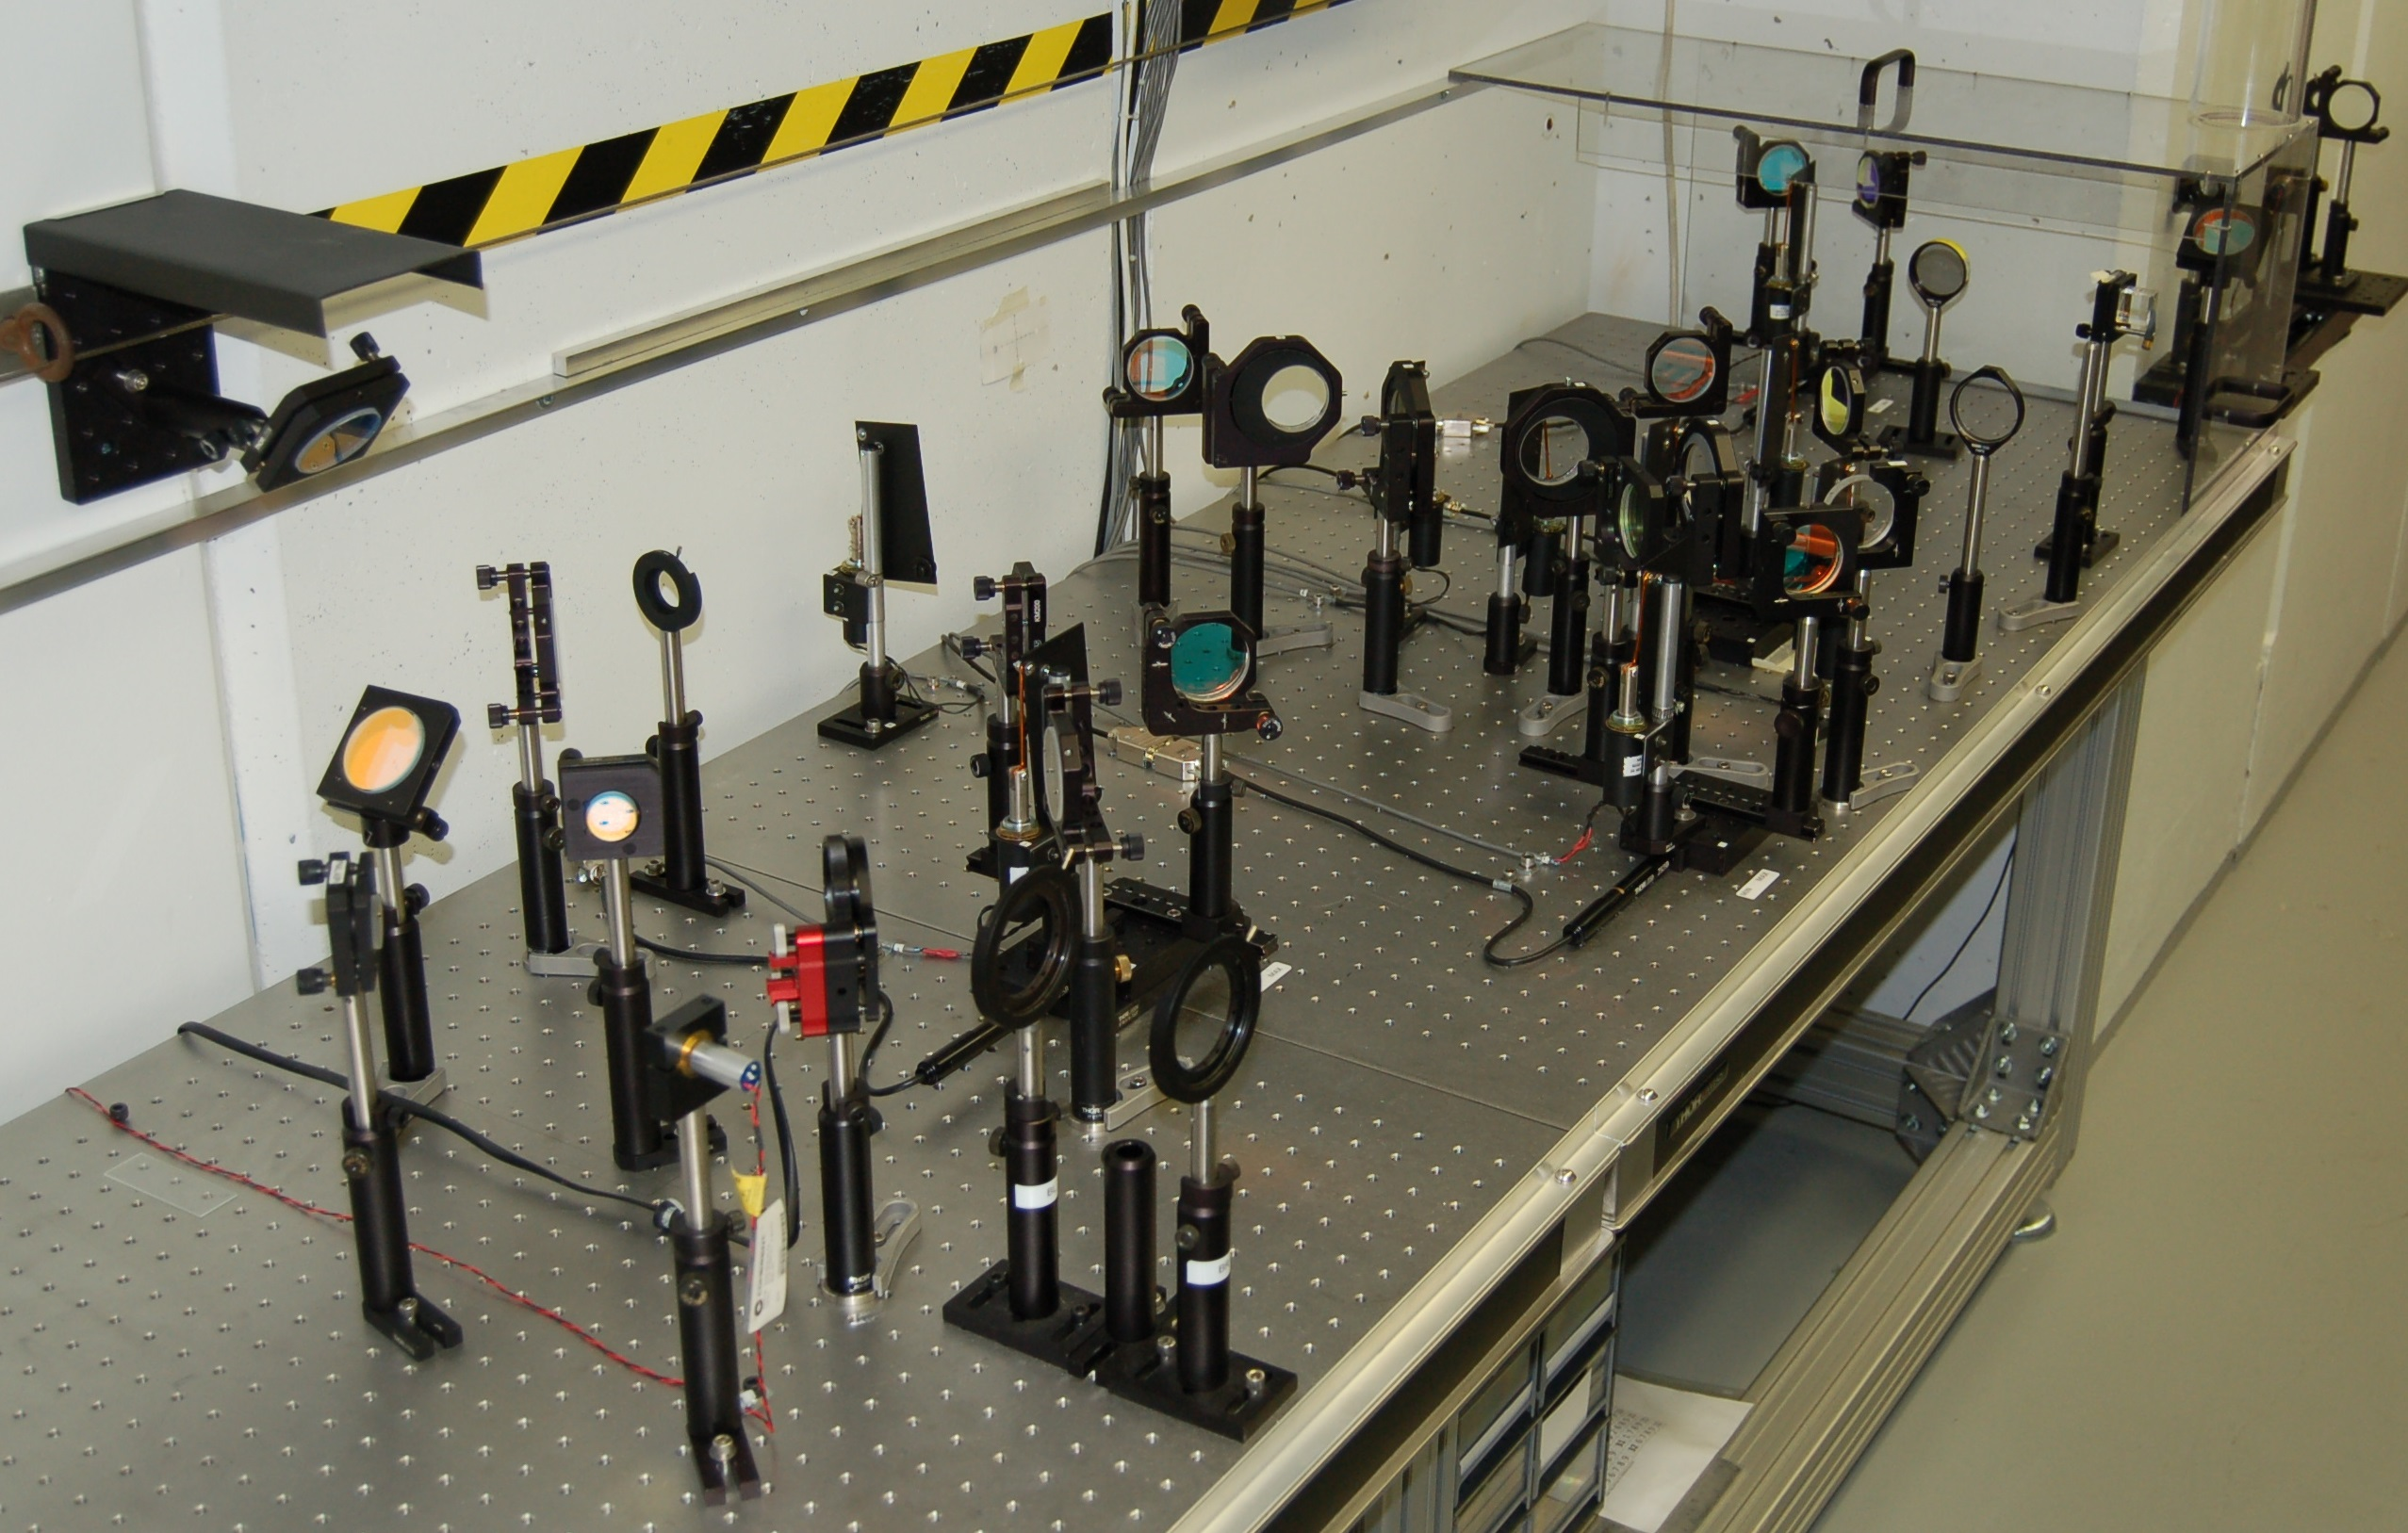
\includegraphics[scale=0.4]{images/multisplitter}\caption{UV Multisplitter optics table.
			The drive gun is located to the right of this table.}
	\end{center}
	\label{fig:multisplit}
\end{figure}
improving the laser pulse train intensity distribution helps
produce an RF power pulse that is closer to uniform. This is key because the generated power depends on both the 
charge and shape of the bunch, as shown in Eq.~\ref{eq:rfpower}. However, as no experiment is perfect, 
several factors contribute to non-uniformity in the bunches. These include the cathode material
(i.e. slightly different QE along the surface), shot to shot noise in the laser pulse, 
distortion due to traveling through air, and the quality of the optics. The last is especially important 
in determining the intensity of each laser pulse in the train.  The UV optics are not perfect, 
meaning each splitter has a slightly different value for transmitted (T) and reflected (R) pulses. 

\Subsection{UV Splitter Measurements} \label{sec:splitmeasure}
Measurements of the UV splitters were done to determine the T/R ratio for 
each splitter. The measurements took place in the laser room, close to the source of the laser.
The setup included two power meters; one to measure the raw T/R values and one to measure 
the background, ASE. This quantity is known to drift with temperature and operating time. 
This is the main contributor to background shot to shot noise in the laser pulse. 
The ASE value was measured when each T/R measurement was taken, then divided out of the T/R 
measurements to prevent bias do to the background drifts. 
Several configurations were tested this way: S-polarization, P-polarization, 
and laser incident on back or front of the coating. Whether the laser pulse hit the front or back of the optic
had no measurable effect on the T/R ratio. Polarization did have a significant effect on
the results, which led to more careful observation of this in the future.
The following plot shows the splitters were performing at about 55/45 ratio, meaning
pulses that were reflected more than one time could have significantly lower intensities than other bunches. 
\begin{figure}[h]
	\begin{center}
		%\includegraphics[scale=0.5]{images/orig_train_intensity}\caption{Original Pulse Train Intensity}
	\end{center}
	\label{fig:origtrain}
\end{figure}

\Subsection{Pulse Train Intensity Measurements} The results in \ref{sec:splitmeasure} predict that
bunches that are transmitted multiple times will contain lower intensity than other
bunches depending on the path through the multisplitter.
by 1$\lambda$ in space by a mirror delay leg. 

\footnote{My Footnote} 

\Section{Kicker}

\Subsection{Kicker Design}

The AWA group does not currently own a kicker, but the theory is well defined. 
A design implemented by Indiana University (IU) \cite{iukicker}
will be adapted to fit TBA requirements at the AWA. Redesign will require optimization
of the length and gap between the kicker plates. Figure \ref{fig:IUkicker} shows the existing IU kicker.
\begin{figure}[h]
	\begin{center}
		%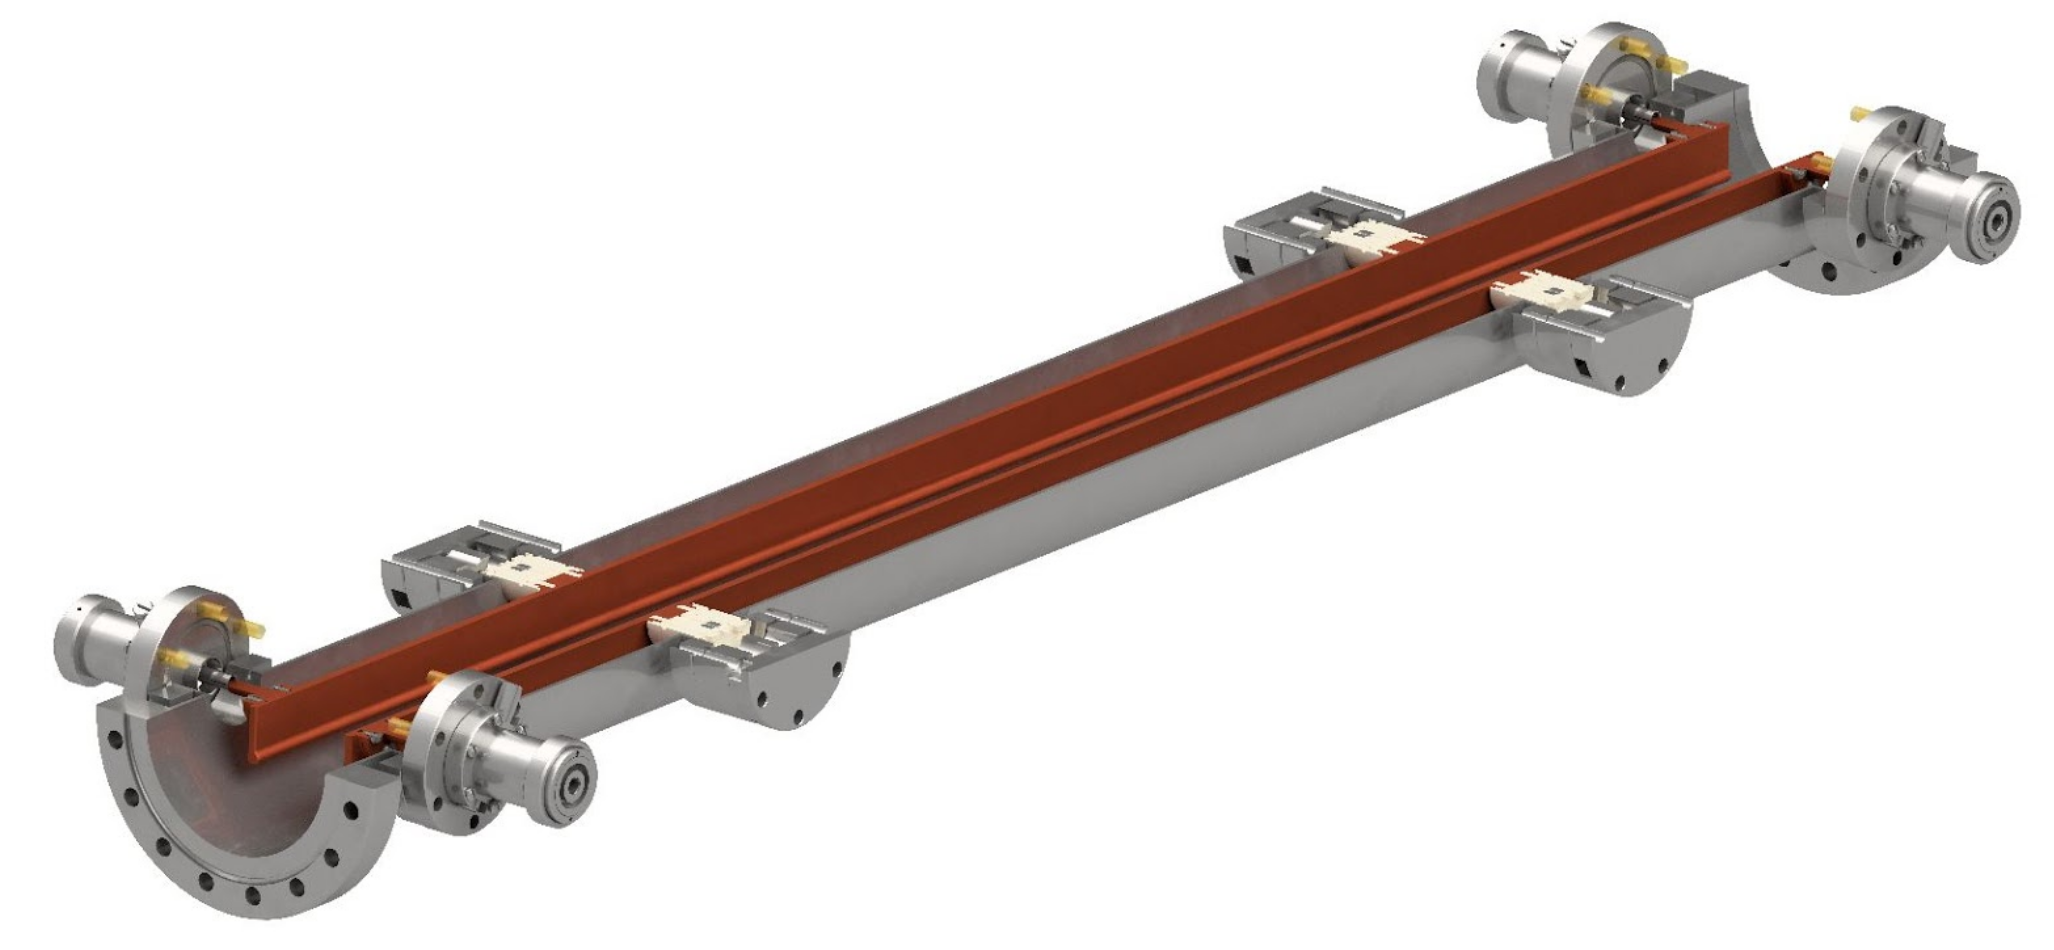
\includegraphics[scale=0.5]{C:/Users/nneveu/Pictures/kicker.jpg}\caption{IU Kicker \cite{IUkicker}}
		\label{fig:IUkicker}
	\end{center}
\end{figure}
The kicker is essentially a parallel plate waveguide. 
A $\pm$35 kV power supply will be used to induce a 70 kV potential difference 
across the plates. Each plate will be terminated in a 50 $\Omega$ load to induce a steady 
state current on the plates. The combination of the two will result in a static TEM mode 
between the plates. Calculation of the electric, $E_v$, and magnetic field, $B_v$,
can be derived from the voltage or current. The electric field, $E_v$, due to a potential, V, is: 
\begin{equation}
E_v=\frac{V}{h}
\end{equation}

Where h is the gap height. From Maxwell's equations, we know that the electric and magnetic 
field are related by the speed of light, c, in the case of plane and TEM waves \cite{pozar}. 
From this we can find the magnetic field induced between the plates: 
\begin{equation}
B_v=\frac{E_v}{c}
\end{equation}
The electrons are going at the speed of light, $c$, and are moving through the kicker on a 
trajectory perpendicular to the fields.  So, it can be seen from the Lorentz force equation, that the force 
exerted on a charge q from the electric and magnetic fields of the TEM mode are equal. 
\begin{equation}
F=q(E_v+v\times B_v)
\end{equation}

Since the force due to the electric field is equal and in the same direction as that from the magnetic field, 
the total kick is just twice that from either field alone.  The angle induced by each field is \cite{iukicker, Wiedemann}:  
\begin{equation}
\theta_E= \frac{V\,L}{h\,T}
\end{equation}
\begin{equation}
\theta_B= \frac{B\,L}{B\rho}
\end{equation}

Where L is the plate length, and T is the kinetic energy of the beam. $B\rho=3.33564\,*T\,$ [GeV-Tesla] is a 
common accelerator physics term that can be found in text such as Wiedemann \cite{Wiedemann}. 
The total angle provided by the kicker is then: 
\begin{equation}
\theta_{total}= \theta_E+\theta_B=2\theta_E=2\theta_B
\end{equation}
From these equations, variable parameters include the gap height, length of the plates, and 
the kinetic energy of the beam. The largest drive beam energy achievable at the AWA is 75 MeV. 
Thesis work will include the optimization of these parameters to obtain the largest angle possible.
Simulations have begun to set boundary conditions on the variable parameters. 

\Subsection{Kicker Installation and Tests}

\Section{Septum Installation} 

\Chapter{Experimental Results} 
\Section{Measurement of Single Stage Power Extraction}
%\Section{Measurement of Single Stage Accelerating Gradient}
%\Section{Measurement of Staged Two Beam Acceleration}


\Chapter{CONCLUSION}
%   \input{Conclusion.tex}
You need a Conclusion.tex file

\Section{Summary}


This was just to create a sample section...

\clearpage


%
% APPENDIX
%
\appendix

\Appendix{Calculations?}

......

%\moretox

\Appendix{OPAL stuff? MCS Stuff?}

Your second appendix text....

\newpage
%
% BIBLIOGRAPHY
%
\bibliographystyle{plain}
\bibliography{thesis}

\end{document}  % end of document





























